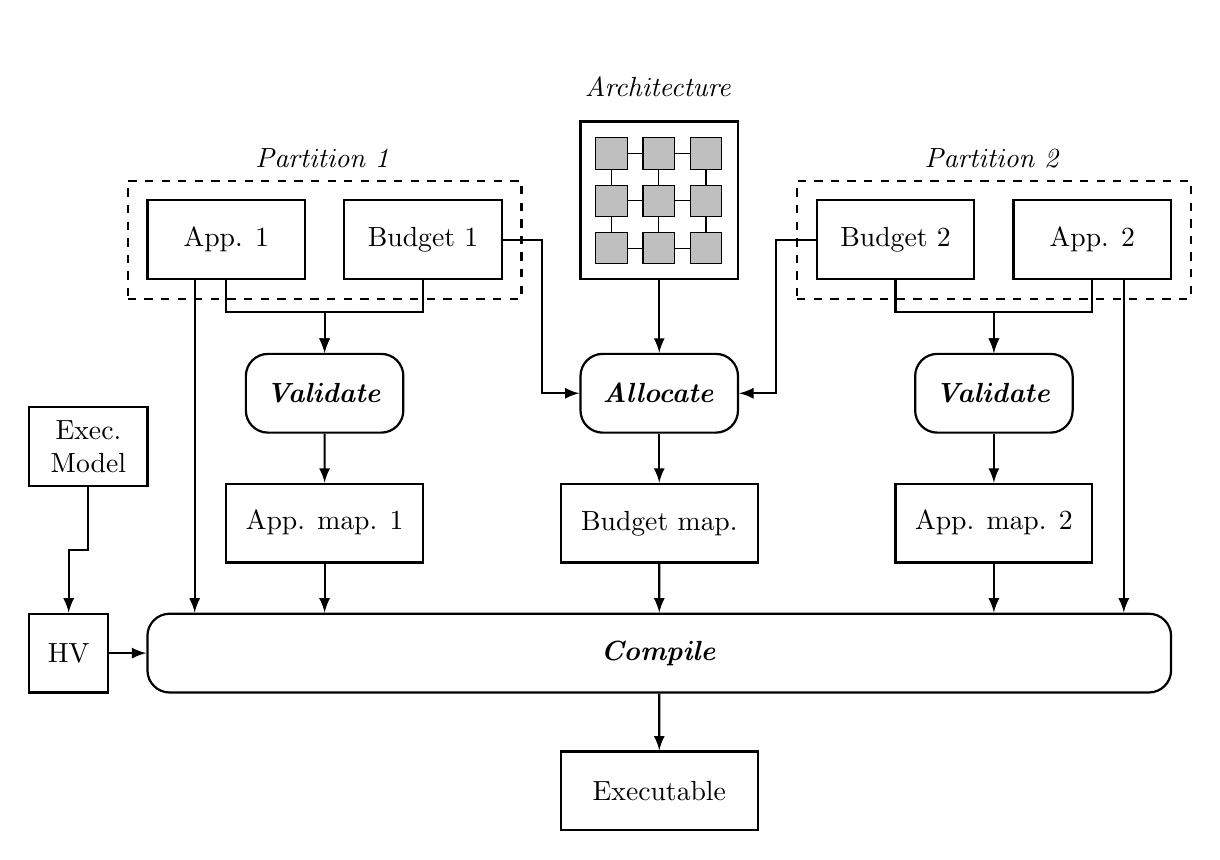
\begin{tikzpicture}
\draw (5.5,0) node[draw, rectangle, inner sep=0pt, minimum width=2cm, minimum height=2cm, anchor=south west, thick] (Archi) {};
\draw (5.7,0.2) node[draw, rectangle, inner sep=0pt, minimum width=0.4cm, minimum height=0.4cm, anchor=south west, fill=lightgray] (t11) {};
\draw (6.3,0.2) node[draw, rectangle, inner sep=0pt, minimum width=0.4cm, minimum height=0.4cm, anchor=south west, fill=lightgray] (t12) {};
\draw (6.9,0.2) node[draw, rectangle, inner sep=0pt, minimum width=0.4cm, minimum height=0.4cm, anchor=south west, fill=lightgray] (t13) {};
\draw (5.7,0.8) node[draw, rectangle, inner sep=0pt, minimum width=0.4cm, minimum height=0.4cm, anchor=south west, fill=lightgray] (t21) {};
\draw (6.3,0.8) node[draw, rectangle, inner sep=0pt, minimum width=0.4cm, minimum height=0.4cm, anchor=south west, fill=lightgray] (t22) {};
\draw (6.9,0.8) node[draw, rectangle, inner sep=0pt, minimum width=0.4cm, minimum height=0.4cm, anchor=south west, fill=lightgray] (t23) {};
\draw (5.7,1.4) node[draw, rectangle, inner sep=0pt, minimum width=0.4cm, minimum height=0.4cm, anchor=south west, fill=lightgray] (t31) {};
\draw (6.3,1.4) node[draw, rectangle, inner sep=0pt, minimum width=0.4cm, minimum height=0.4cm, anchor=south west, fill=lightgray] (t32) {};
\draw (6.9,1.4) node[draw, rectangle, inner sep=0pt, minimum width=0.4cm, minimum height=0.4cm, anchor=south west, fill=lightgray] (t33) {};
\draw (t11) -- (t12) -- (t13); 
\draw (t21) -- (t22) -- (t23); 
\draw (t31) -- (t32) -- (t33); 
\draw (t11) -- (t21) -- (t31); 
\draw (t12) -- (t22) -- (t32); 
\draw (t13) -- (t23) -- (t33); 

\draw (5.5,1.7) node[inner sep=0pt, minimum width=2cm, minimum height=1.5cm, anchor=south west] {\textit{Architecture}};

\draw (0,0) node[draw, rectangle, inner sep=0pt, minimum width=2cm, minimum height=1cm, anchor=south west, thick] (App1) {App. 1};
\draw (2.5,0) node[draw, rectangle, inner sep=0pt, minimum width=2cm, minimum height=1cm, anchor=south west, thick] (Bud1) {Budget 1};
\draw (8.5,0) node[draw, rectangle, inner sep=0pt, minimum width=2cm, minimum height=1cm, anchor=south west, thick] (Bud2) {Budget 2};
\draw (11,0) node[draw, rectangle, inner sep=0pt, minimum width=2cm, minimum height=1cm, anchor=south west, thick] (App2) {App. 2};

\draw (-0.25,-0.25) node[draw, rectangle, inner sep=0pt, minimum width=5cm, minimum height=1.5cm, anchor=south west, thick, dashed] {};
\draw (-0.25,0.8) node[inner sep=0pt, minimum width=5cm, minimum height=1.5cm, anchor=south west] {\textit{Partition 1}};
\draw (8.25,-0.25) node[draw, rectangle, inner sep=0pt, minimum width=5cm, minimum height=1.5cm, anchor=south west, thick, dashed] {};
\draw (8.25,0.8) node[inner sep=0pt, minimum width=5cm, minimum height=1.5cm, anchor=south west] {\textit{Partition 2}};

\draw (5.5,-1.95) node[draw, rectangle, inner sep=0pt, minimum width=2cm, minimum height=1cm, anchor=south west, rounded corners=8pt, thick] (Alloc) { \textbf{\textit{Allocate}}};
\draw (1.25,-1.95) node[draw, rectangle, inner sep=0pt, minimum width=2cm, minimum height=1cm, anchor=south west, rounded corners=8pt, thick] (Valid1) {\textbf{\textit{Validate}}};
\draw (9.75,-1.95) node[draw, rectangle, inner sep=0pt, minimum width=2cm, minimum height=1cm, anchor=south west, rounded corners=8pt, thick] (Valid2) {\textbf{\textit{Validate}}};

\draw[-latex, thick] (App1.south) -- ([yshift=-4mm]App1.south) -| (Valid1.north);
\draw[-latex, thick] (Bud1.south) -- ([yshift=-4mm]Bud1.south) -| (Valid1.north);
\draw[-latex, thick] (App2.south) -- ([yshift=-4mm]App2.south) -| (Valid2.north);
\draw[-latex, thick] (Bud2.south) -- ([yshift=-4mm]Bud2.south) -| (Valid2.north);
\draw[-latex, thick] (Bud1.east) -- ([xshift=5mm]Bud1.east) |- (Alloc.west);
\draw[-latex, thick] (Bud2.west) -- ([xshift=-5mm]Bud2.west) |- (Alloc.east);
\draw[-latex, thick] (Archi.south) --  (Alloc.north);

\draw (1,-3.6) node[draw, rectangle, inner sep=0pt, minimum width=2.5cm, minimum height=1cm, anchor=south west, thick] (AppMap1) {App. map. 1};
\draw (5.25,-3.6) node[draw, rectangle, inner sep=0pt, minimum width=2.5cm, minimum height=1cm, anchor=south west, thick] (BudMap) {Budget map.};
\draw (9.5,-3.6) node[draw, rectangle, inner sep=0pt, minimum width=2.5cm, minimum height=1cm, anchor=south west, thick] (AppMap2) {App. map. 2};

\draw[-latex, thick] (Valid1.south) --  (AppMap1.north);
\draw[-latex, thick] (Valid2.south) --  (AppMap2.north);
\draw[-latex, thick] (Alloc.south) --  (BudMap.north);    

\draw (-1.5,-2.625) node[draw, rectangle, inner sep=0pt, minimum width=1.5cm, minimum height=1cm, anchor=south west, text width=1.25cm, align=center, thick] (EM) {Exec. \\ Model};

\draw (-1.5,-5.25) node[draw, rectangle, inner sep=0pt, minimum width=1cm, minimum height=1cm, anchor=south west, thick] (HV) {HV};

\draw[-latex, thick] (EM.south) -- ([yshift=-8mm]EM.south) -| (HV.north);

\draw (0,-5.25) node[draw, rectangle, inner sep=0pt, minimum width=13cm, minimum height=1cm, anchor=south west, rounded corners=8pt, thick] (Compile) {\textbf{\textit{Compile}}};

\draw[-latex, thick] (AppMap1.south) --  (AppMap1|-Compile.north);
\draw[-latex, thick] (AppMap2.south) --  (AppMap2|-Compile.north);
\draw[-latex, thick] (BudMap.south) --  (Compile.north);
\draw[-latex, thick] ([xshift=-4mm]App1.south) --  ([xshift=-4mm]App1.south|-Compile.north);
\draw[-latex, thick] ([xshift=4mm]App2.south) --  ([xshift=4mm]App2.south|-Compile.north);
\draw[-latex, thick] (HV.east) --  (Compile.west);

\draw (5.25,-7) node[draw, rectangle, inner sep=0pt, minimum width=2.5cm, minimum height=1cm, anchor=south west, thick] (exec) {Executable};
\draw[-latex, thick] (Compile.south) --  (exec.north);


\end{tikzpicture}

